\documentclass[letterpaper]{book}

\usepackage[fontset=fandol]{ctex}
\usepackage{titlesec}
% 每节换新页
\newcommand{\sectionbreak}{\newpage}
\usepackage[utf8]{inputenc}
\usepackage[singlelinecheck=false]{caption}
\usepackage{amsmath}
\usepackage{amsfonts}
\usepackage{graphicx}
\usepackage{mathrsfs}
\usepackage{xeCJK}
\usepackage{color}
\usepackage[colorlinks,
linkcolor=magenta,
anchorcolor=red,
citecolor=blue]{hyperref}
\usepackage{url}
\usepackage{listings}
\usepackage{shortvrb}
\usepackage{stfloats}
\usepackage{bigstrut}
\usepackage{wallpaper} %使用wallpaper宏包
\CenterWallPaper{}{img/paper}
\usepackage[inner=3cm,outer=1.5cm]{geometry}
\MakeShortVerb{|}

\title{终极笔记 \\ Research Note}
\author{修格致}
\date{2020年4月6日-\today}

\begin{document}

\frontmatter

\maketitle

\tableofcontents

\mainmatter

\chapter{序言}

\paragraph{序章:} 本书是我从博二下半年开始的文献笔记和idea拾遗。会十分不连贯,不过也不乏精彩的部分。这已经是我第二年的下半年了。而我仍然觉得觉得距离第一年并没有过去多久,一切还是开始时的样子。希望回头看看时,已经做成了自己想做的工作!


\section{关于}
\textcolor[rgb]{0,0,1}{更新于2020年4月6日。}

现在我的研究兴趣集中在城市生态系统、城市韧性、以及相关的数学物理模型上。本文的主要内容也将是涉及这些内容。这个过程大概将持续到2021年的7月,作为我心目中博士阶段的三块基石中的第一块。

\subsection{空间流行病学}
2020年是个地狱开局。大卫·斯特恩和科比布莱恩特去世了。紧接着COVID走入并改变了我们每个人的生活。这个时候我们没有人可以置身事外。我也想做一些有意义的相关研究。我不希望我这些研究仅仅是涉及本次疫情的特定情况。更重要的是我们如何在每次流行病发生的时候应对得好一点,再好一点。

\subsubsection{流行病传播的时空特征}
工具:
\begin{itemize}
    \item 小波分析
\end{itemize}

%%%%%%%%%%%%%%%%%%%%%%%%%%%%
\chapter{空间流行病学}

代表作家:Grenfell、Durrett(\href{https://services.math.duke.edu/~rtd/Talks/Talks.html}{近期演讲主页},\href{https://services.math.duke.edu/~rtd/survey/survhome.html}{Stochastic Spatial Models: A Hyper-Tutorial})

\begin{quote}
    You won't stop it until you fully understand it. It won't just \textit{magically} disappear.
\end{quote}



\section{时空传播规律}
重要文献:Travelling waves and spatial hierarchies in measles epidemics, Bryan Grenfell et. al., Nature 2001

\paragraph{流行病传播的实际问题与理论模型的区别} |实际问题|: 要注意流行病的具体传播规律。不光是参数的设定,更是大类模型的选择。要关注非线性、时空异质性、非马氏性等重要因素。

\subsection{孤立人口中流行病传播的幂律分布}

\href{https://www.nature.com/articles/381600a0}{Power laws governing epidemics in isolated populations, C. J. Rhodes and R. M. Anderson}

在生物时间序列中非线性和混沌模式的识别和分析的背景下,发达国家\textbf{大型城市}社区中麻疹病毒感染的时空变化一直是许多讨论的焦点。 相反,由于感染记录的频繁消失且高度不规则,孤立的小岛屿人群用传统分析并不能提供有用的见解。本文使用流行病大小和持续时间分布的方式来证明这种系统动力学的\textbf{规律性}(regularities)是明显的。 具体而言,这些生物学系统的特征是定义明确的幂律分布,其方式类似于物理学中其他非线性的,空间中展开的动态系统。本文进一步表明,所观察到的幂律指数已通过基于网格的简单模型很好地描述,该模型反映了各个宿主之间的社会交互。

人口学上来讲,小岛上的现象通常可以不考虑与外界的交互,从而是一个良好的社区化语境。法罗群岛(知乎链接:\href{https://zhuanlan.zhihu.com/p/26426579}{法罗群岛的绞肉机},讲得是这个地方的大家去捕鲸的故事)是丹麦的海外自治领地。地理位置介乎挪威海和北大西洋中间,处于挪威到冰岛之间距离一半的位置。

法罗群岛的人口总数为25,000。外部人口与之交互会带来流行病麻疹。我们认为输入病例是非常精确的,因为法罗群岛面积小而交互局部化,也因为每个病例在这里都会引起很大重视。在58年中,有43个互不相同的epidemic event(\textbf{定义}为连续的$t = \tau_{\text{end}}-\tau_{\text{start}}$个月都出现有限个病例记录,这段时间的前后月份都不出现麻疹病例)。每个event的规模(size)定义为病例数的求和:$s = \sum_{\tau_{\text{start}}}^{\tau_{\text{end}}} C(\tau)$.地震学里面有个\href{https://www.nature.com/articles/nature04094}{Gutenberg-Richer定律},说的是地震频率与烈度之间关系的幂律分布,长得就跟法罗群岛流行病的发病情况差不多,都是$\log N(>s) = a-b\log s$。流行病的频数和持续时间的幂律关系在本文找到了:\begin{align}
    &N(s) \propto s^{-1-b}, &b\simeq 0.28\\
    &N(t) \propto s^{-1-c}, &c\simeq 0.8
\end{align}这两个关系对我们估计短期内流行病规模和持续时间的概率分布是十分有用的。小而短的麻疹疫情比大而长的麻疹疫情要更频繁出现。这种幂律关系的好处是它对子样本数据同样成立,可以用前一半数据来预测后一半数据。作者利用博恩霍尔姆岛和雷克雅未克的精确麻疹病例来估计来幂律指数$b$和$c$。连同法罗群岛,这三个地方的幂律指数是高度吻合的。

这种幂律现象为什么会出现还不能很好的被理解。有一些作者没有提到的空间模型做得还不错。于是作者使用了一个基于格点的模型,该模型之前被用为\textit{林火传播}的模型,用在这个空间\textit{S-I}的场景也合适(相关文献:\href{https://journals.aps.org/prl/abstract/10.1103/PhysRevLett.69.1629}{phys. rev. lett. 自组织临界的林火模型}、\href{https://journals.aps.org/pre/abstract/10.1103/PhysRevE.55.2174}{phys. rev. e 林火模型中的相变}、\href{https://journals.aps.org/pre/abstract/10.1103/PhysRevE.50.1009}{phys. rev. e 林火模型的标度律和模拟结果} 这几个是同一个团队的作品)。\textbf{模型叙述如下}:periodic的离散的$L\times L$格点图上,每个点有三种可能的状态:被感染、易感、空点,随着离散的时间更新。更新规则是:

\begin{enumerate}
    \item 如果易感者S的最近邻居有患者,就可能被感染;
    \item 患者I失去活性,所处位置清空;
    \item 易感者以概率为$\mu$移动到空格子上;
    \item 新患者I不时以概率$\gamma$被感染。
\end{enumerate}

模型有效反映了代表罕见外来病例作用的迁移项。模拟用$L = 250$, $\mu = 2.6\times 10^{-5}$, $\nu = \mu/300$, 得到了$b\simeq 0.29$, $c\simeq 1.5$的结果。模型对十个月以上的长期流行病的数量是低估的。网络模型的占用情况可以模拟真实社区。平均人口密度是$25,000$,这意味着每$4$个位置有一个人。均衡状态下,平均寿命如果是$70$岁,我们期望每天有$\sim 1$个新生儿降生。真实的$\nu/\mu$应该是$1/400$,而不是模拟使用的$1/300$. 新生的易感人群和患病的人的迁移由均值为$1$和$1/300$泊松过程刻画,这样一个step相当于一天。模拟结果受长期误差影响非常大,但是对5个月以内的流行病的分布有着很好的复现。

作者还使用了随机SEIR模型进行对比。此时人口被假设为均匀同质混合,外来人口比例很低。同样计算了时间和规模的分布。这个模型高估了大流行病的频率,而且与真实分布吻合不好。SEIR模型很可能不适合小人口的不频繁的流行病。

我们的结果表明,在孤立的海岛麻疹数据集中存在流行病的规模和持续时间的标度律。这将这些流行病的动力学与其他空间扩展的非线性动力学系统归为同一类,在该非线性动力学系统中也观察到标度律。实际上,这促进了一种预测方法,可以计算给定大小和持续时间的流行病的发生频率。

一个简单的空间模型所产生的指数几乎与我们的数据分析所见的相同。幂律现象也可能与高度接种疫苗的社区和发展中国家偏远农村人口中麻疹不经常爆发的研究有关。这里讨论的方法是完全通用的,可以应用于少数人群中任何其他时间序列的传染病暴发。
    
\href{https://science.sciencemag.org/content/sci/312/5772/447.full.pdf}{Synchrony, Waves, and Spatial Hierarchies in the Spread of Influenza}

量化流行病的长程传播是疾病动力学和疾病控制的主要因素。本文使用美国超过30年(1972-2002)流感周期数据来分析两次爆发之间变化规律。流感高发季度的传播能力更快更强。

\subsection{跨尺度人口动力学得共生吸引子:伦敦的麻诊病例}

这是Grenfell 2020年的论文。

\textit{大城市人口中麻疹传染的模式通常被认为是一个同步的非线性动态模式。确实,虽说能看出一些异质性,疫情还是循环往复地出现,而且很接近mass-action模式。但是使用一个1897-1906年的死亡数据集,我们对这个假设提出了挑战。我们发现,伦敦的一个区域体现出单双年周期混合的模式,尽管全市范围内,疫情周期是一整年。使用一个简单的随机流行病传播模型和最大似然推断的方法,我们证明我们可以获取这个变化的周期。我们的理论与数据是一致的,这表明时间上的周期性与空间上的局部关联都符合简单规律。特别的,我们发现季节导致的局部变化驱动了周期性。我们的结果表明,强混合人口中,有很多的吸引子共存。理论上这些吸引子都是可以解释的。}

\paragraph{数据}

伦敦的五个内城区(小)和四个外城区(大,称为东西南北)。每周的麻疹死亡记录,每年的人口统计、每年新生儿数的\textbf{数据来源}:Registrar General's reports(\href{1897 Weekly return of birth and deaths in London and other great towns}{https://catalog.hathitrust.org/Record/012306663})。死亡数据实际上聚合到了每四周为一个单位,来增强周期性的信号。年度出生率被插值到了月度,来平滑参数估计。麻疹的周期使用谱密度波峰的最近整数周期法来估计。

\paragraph{理论模型}

随机SEIR模型+周期传染率, $\beta(t) = \bar{\beta(1 + \alpha \sin(2\pi t +\phi)}$. 

\paragraph{推断框架}

要推断的是 time-invariant case fatality rate (CFR), 假设死亡被完全统计进来了,这也就是一个不完美观测的一个相对度量。

还要估计一个平均输入率 $\iota$, 这个参数的意义是防止随机灭绝。

对于125个月的小样本,为了防止过拟合,假定潜伏期和感染期分别为8天和5天。由\textbf{迭代过滤算法},来逐个区域地估计stochastic SEIR模型的参数。这种方法的容错是比较好的,可以在参数空间random walk直到得到最大似然估计。(不过需要迭代很多次)得到参数的最大似然估计之后,就可以用模型预测未来的结果并与实际情况比对了。

\subsubsection{隐含理论背景}



\section{大空间尺度的地理学问题}

\href{https://www.nature.com/articles/414716a.pdf}{麻疹传播的波状结构和空间层次}时空行波是捕食者-猎物和宿主-寄生虫动力学的显着表现。然而,很少有系统的文献足以检测重复的波并解释它们与人口结构和人口统计学的时空变化的相互作用。在这里,我们用详尽的时空数据集证明了英格兰和威尔士的流行性流行行波。我们使用小波相位分析,可以实现动态非平稳性-解释这些以及其他许多生态时间序列中的时空模式很复杂。在疫苗接种之前的时期,明显的分层感染浪潮从大城市向小城镇转移。麻疹疫苗的引入限制,但并没有消除这种等级传染病。一个机理上的随机模型为从大的“核心”城市到较小的“卫星”城镇通过传染性“火花”传播的海浪提供了动力学解释。因此,宿主种群结构的空间层次是这些感染浪潮的先决条件。

旅行波来自于激活-抑制动力学研究,并被很多的host-natural enemy 系统所预测。但是除了入侵动力学,经验观测被研究的还是比较少。

\subsection{麻疹行波的强迫林火模型}



\subsection{from individuals to epidemics}
\chapter{网络弹性}
\chapter{演化网络}

\section{Essentials}

\subsection{防范意识对随机网络上的疾病传播的影响}
\href{https://www.sciencedirect.com/science/article/pii/S002251931930459X}{防范意识对随机网络上的疾病传播的影响}。文章中说流行病\textit{期间}产生的防范意识不会对basic reproduction number产生影响。从其他人群中产生的防范意识会降低$R_0$. 防范意识可以显著减小流行病的规模,切断与病人的连边比降低感染率的效果要明显得多。流行病规模不会随着防范意识和感染率单调减小。局部和全局的防范意识是否对流行病规模产生影响取决于网络的类型和感染率。

\subsection{偏好与地理对流行病传播的影响}
\href{https://journals.aps.org/pre/abstract/10.1103/PhysRevE.76.056109}{偏好与地理对流行病传播的影响}:随机网络上的SIS模型,每个时刻,空间网络增加一个有$m$条边的结点。它与度为$k_{j}$,距离为$d_{ij}$的结点$j$连接的概率正比于$k^{A}_{j}/d^{B}_{ij}$, $A$和$B$都是正常数。如果$A=0$, 就是有临界值的普通疾病传播,疾病最终会消失;$B=0$时,(a) $A=1$时没有临界行为,其他时候仍然有临界行为。如果两个因素同时存在,临界值之上的~$A$和临界值之下的~$B$控制的网络对于传染是有鲁棒性的。

\subsection{Epidemic thresholds in dynamic contact networks}
\href{https://royalsocietypublishing.org/doi/pdf/10.1098/rsif.2008.0218}{Epidemic thresholds in dynamic contact networks}再生率$R_0$是流行病学中的基本量,它决定了易感群体中传染病的一阶增长。在大多数流行病的\textbf{理论模型}中,都有一个特定的值$R_0$,即流行病阈值,高于该值可能会大流行,但低于此值就不会发生大流行。随着流行病模型的复杂性增加,计算流行病阈值的难度也增加。本文通过简单的动态随机网络类推导了SIR流行病的$R_0$和流行阈值。与大多数流行病学模型一样,$R_0$取决于两个基本流行病参数,即传播率和恢复率。我们发现,$R_0$还取决于社会参数,即描述并发联系人数量异质性的\textbf{度分布}以及给出联系人启动和终止速率的混合参数。我们表明,社会融合从根本上改变了流行病学格局,因此,用静态网络来近似动态网络可能是不足够的。

几个简写:neighbour exchanges (NEs)

任意度分布的静态随机网络已经有很多研究在做了(Callaway et al. 2001; Newman et al. 2001, 2002; Chung \& Lu 2002; Catanzaro et al. 2005)。我们假设一个度分布为$\{p_k\}$的网络。对于大型的网络,给定一条ego到$x$边,$x=alter$的概率正比于alter的度。用 $\{ego, alter\}$来记录一条边; $(ego, alter)$ 来记录ego到alt的联系。

\section{随机图上疾病和信息的传播}

\href{https://www.pnas.org/content/pnas/107/10/4491.full.pdf}{Some features of the spread of epidemics and information on a random graph}. 

\paragraph{三种随机图}\textbf{小世界}图是Watts和Strogatz引入的。在一维圆环$\mathbf{Z} ~\text{mod}~n$上,连接所有距离小于等于$m$的点。然后以概率$p$,将边的一端连到纯随机的另一个结点上。\textbf{BA模型}依次加入结点,连接$m$条边到已有结点上,概率正比于该结点的度。该模型的度分布收敛于\begin{equation} p_{k}=\frac{2 m(m+1)}{k(k+1)(k+2)} \quad \text { for } k \geq m \end{equation}如果不是正比于度,而是一个平移项$k+a$ ($a>-1$), 那么度分布将会是$p_k\sim C k^{-3+a}$. 如果$a\geq 0$, 这种方式等价于:新边以概率为$a/(a+1)$随机选一个结点,以概率为$1/(a+1)$使用偏好依附机制。\textbf{NSW模型},给定度分布$\{p_k,k\geq 0\}$, 独立采样出真实的度序列$\{d_k\}_{k=1,\dots, n}$, 假设采样出的度的和为偶数,然后结点依次随机连$d_i$条边,构建一个$n$个结点的随机图$G_{n}$. 

\paragraph{两种流行病}\textbf{SIR}类似于分枝过程,以速率为$\lambda$感染,以速率为$1$恢复,恢复之后不易感。该模型与渗流模型有很好的对应。如果$x$, $y$在图里是邻居,就以概率为$\lambda/(\lambda+1)$, 也就是二者之一患病期间感染另一人的概率,连边。流行病的规模就是含有初始被感染结点的连通图的大小。\textbf{SIS}模型要更复杂一些。感染和恢复速率分别是$\lambda$和$1$. 这又称为\textit{接触过程}。

\textbf{小世界网络}的简单版本$m=1$在Watts和Strogatz的小世界十年前就被Bollobas和Chung提出了。这种小世界的半径是$\sim\log_2 n$. 称为BC小世界。我们希望每个个体有且只有一个长程联系,这样就可以定一个相关的大世界图$\mathscr{B}_m$. 

自由积是个不错的形式。$\mathbf{Z}*\{0,1\}$. 其中的元素的形式是$z_01z_11\dots 1z_k$. 也就是移动$z_0$连到$1$, 然后到$z_{1}$再到$1$以此类推。这个文章太难了我以后再看吧。不过真的好精彩。

\href{https://journals.aps.org/pre/pdf/10.1103/PhysRevE.82.036112}{演化网络上的疾病传播}

\subsection{适定性网络上的流行病动态}
\href{https://journals.aps.org/prl/abstract/10.1103/PhysRevLett.96.208701}{Epidemic Dynamics on an Adaptive Network}

易感者能够通过重新连接其网络连接来避免与感染者接触。引起、分类度相关性,振荡,磁滞和一阶跃迁。

考虑例如在社交网络上传染病的传播。人类倾向于通过\textbf{避免与感染者接触}来应对这种流行病。局部连接的这种重新布线可对疾病的动力学产生强烈影响,进而影响重新布线过程。因此,出现了时变网络拓扑与节点动态之间的复杂交互。自适应网络上的SIS模型可以证明,用于网络连接的简单直观的重连规则对网络具有深远的影响,并且能够生成特定的网络属性,例如广度分布,分类度相关性以及两个松散连接的子隔间的形成。\textbf{动力学上的结果}是出现了新的流行阈值(对应于一阶跃迁),多个稳定平衡的共存(导致磁滞)以及振荡机制的出现,所有这些在静态SIS网络中都是不存在的。

考虑结点数为 $N$, 边数为 $K$ 的网络上的SIS过程。每个时间节点上,每个S-I边以概率 $p$ 变成I-I;每个I以概率为 $r$  恢复健康。\textbf{重连}体现在:S可以通过重连来保护自己。SI以概率为 $w$ 被打断,连接到一个随机的健康S结点。

\paragraph{流行条件}考虑临界感染概率$p^*$. 在不重连的网络上,基本再生数$R_{0}:=p\langle k\rangle / r$, 其中 $\langle k\rangle=2 K / N$,它表示由其他易受感染的网络上的单个感染节点引起的继发感染数。所以,给定网络结构,需要一个二级感染的话,$p^* = t/\langle k \rangle$. 如果考虑网络重连的话,一个 I 结点平均每次会失去 $w$ 比例的邻居。邻居数将是 $k(t)=\langle k\rangle \exp (-w t)$. 由于 I 的周期时$1/r$, 阈值将是\begin{equation}
    p^{*}=\frac{w}{\langle k\rangle[1-\exp (-w / r)]}\label{eq:rewire_threshold}
\end{equation}
由于$w\gg r$时,$p^* = w/\langle k\rangle$, 所以高重连率会使得流行病阈值提高很多,进而减小流行病的程度。

分几种情况:

\paragraph{重连与状态独立}

度分布是泊松分布,给定结点二阶邻居的平均度 $\langle k_{nn} \rangle$ 与度 $k$ 是独立的。

\paragraph{上面的重连规则}

先让SIS机制关掉,即 $r = p = 0$. 设 I 的比例是 $i$, $S$ 的比例是 $s = 1-i$, 都是常数。但是 SI 边随时间不断减少,逐渐变成不在一起的两个组团。假设我们从一个随机图开始,各种类型边的密度分别是 $l_{SS}=s^2\langle k\rangle /2 $, $l_{II}=i^2\langle k\rangle /2 $, $l_{SI}= \langle k\rangle /2 - l_{II} - l_{SS} = si\langle k\rangle $. 有适定性重连规则之后,稳定状态下所有的 SI 边都会转为 SS 边,密度是 $l_{SS} = (1-i^2)\langle k \rangle/2$. 因此,S 与 I 在不同的度分布 $\rho_k$ 假定下,S 的平均度 $\langle k_S \rangle = (1+i)\langle k\rangle $, I 的平均度 $\langle k_I \rangle = i\langle k_I \rangle$. 虽然各自还是泊松的,但是 S 组团的联通度更高。由于 $ \langle k_{nn} \rangle$ 与两个集团中分别的度 $k$ 都是独立的,组团内部的度关联也消失了。但是如果两个组团考虑在一起,一个\textit{净度关联} $r_\text{corr} > 0$ 可以出现,因为 $\langle k_{nn} \rangle$ 对于 S 组团更大。

\begin{figure}
    \centering
    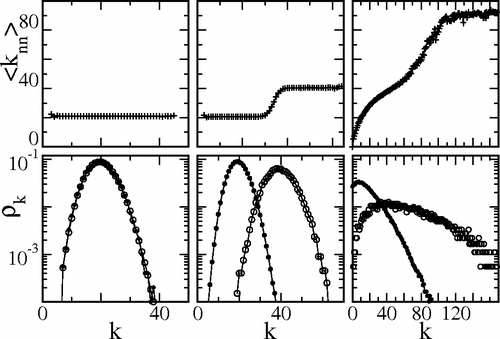
\includegraphics[width = 0.5\linewidth]{Pics/rewire-structure-of-adaptive-networks.png}
    \caption{适定性网络的结构。上边一行是平均最近邻度$\langle k_{nn} \rangle$, 下面一行是度分布。从左到右分别是无差别重连/没有SIS关系的/适定性网络。参数设置是$w = 0.3$, $r = 0.002$, $p = 0.008$, $N = 10^5$, $K = 10^6$.}\label{fig:rewire-structure}
\end{figure}

最后,同时考虑适定性重连与流行病动力。虽然重连没有快到可以完全分离 S 与 I,但是还是能形成两个比较松散连接的组团,比如说 $l_{SI} \approx 0.01\langle k \rangle$. 组团间联系在被切断,有的 I 结点也在康复,有的 S 结点也在被感染。这导致结点度随时间的巨大变化。只要一个结点是 S,它的度几乎就以线性增长,\begin{equation}
    \dot{k} = wl_{SI}.
\end{equation} 反之,感染的结点的度以指数递减,\begin{equation}
    \dot{k} \sim -wk.
\end{equation}所以存在一个复杂的均衡,组团间和组团内的边,S 与 I 的密度都是一个常数。这个均衡中,连续的重连会维护一组 S 与 I 的度分布,以及一个正的度关联(高高相连,低低相连)。

\paragraph{进一步的性质}
\begin{figure}
    \centering
    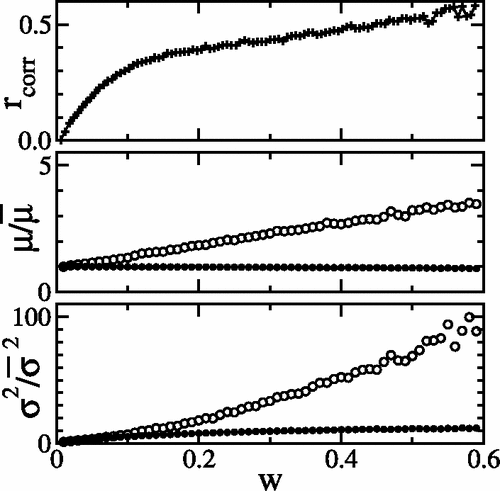
\includegraphics[width = 0.5\linewidth]{Pics/Degree_correlation_index.png}
    \caption{上图是$r_\text{corr}$作为$w$的函数,下图是度分布的均值和方差作为$w$的函数。空心是 S,实心是 I. 都相对于没重连的情况标准化了。参数是$N=10^5$, $K = 10^6$, $r = 0.002$, $p = 0.008$.}\label{fig:parameters_vs_rewire}
\end{figure}

图~\ref{fig:parameters_vs_rewire}~进一步量化了自适应重新布线对新兴网络结构的影响。随着$w$的增加,相关度迅速增加。此外,易感者的平均程度增加而感染程度则略有下降。甚至更明显是在易感的度分布的方差的增加。比如$w=0.6$时的方差$\sigma^2$大了100倍。这表明形成了牢固连接的中心和临时孤立的节点,这些节点由重连而迅速重新连接。

适应性重连促进了受感染个体的隔离,这可以大大提高流行阈值。然而,这样做时,连引入了人口中连接的混合,并且还导致形成高度连接的易感簇,其特征在于度分布的方差较大,因此具有较低的流行阈值。因此,重连的局部作用趋于抑制流行,而产生的拓扑作用则促进流行。所以重连有两个相反的作用。

为了研究这个问题,我们考虑一个低维问题中的 $l_{SS}$ 和 $l_{II}$. 利用moment closure approximation方法。对于$a,b,c\in[S,I]$做如下近似:$l_{abc} = l_{ab} l_{bc} / b$. 这样的系统上面就有如下的ODE:
\begin{align}
    \frac{d}{d t} i&=p l_{\mathrm{SI}}-r i\\
    \frac{d}{d t} l_{\mathrm{II}}&=p l_{\mathrm{SI}}\left(\frac{l_{\mathrm{SI}}}{s}+1\right)-2 r l_{\mathrm{II}}\\
    \frac{d}{d t} l_{\mathrm{SS}}&=(r+w) l_{\mathrm{SI}}-\frac{2 p l_{\mathrm{SI}} l_{\mathrm{SS}}}{s}
\end{align}
它可以与数值模拟的结果,也就是图~\ref{fig:bifurcation_diagram}。在不重新布线的情况下,只有一个连续的动态过渡发生在流行阈值$p^∗$上。随着重连,该阈值与等式~\ref{eq:rewire_threshold}完全吻合。但同时,也会出现\textbf{一个较低的鞍点分叉}。该点之上,已有的流行病会继续存在。与没有重连相比,两个流行病机制之间出现了不连续一阶相变(导数就不连续了)。其之间有双稳定状态,健康和流行病可能都是稳定的。所以,会形成一个\href{https://baike.baidu.com/item/滞后回线/360581?fr=aladdin}{滞后曲线}。

\begin{figure}
    \centering
    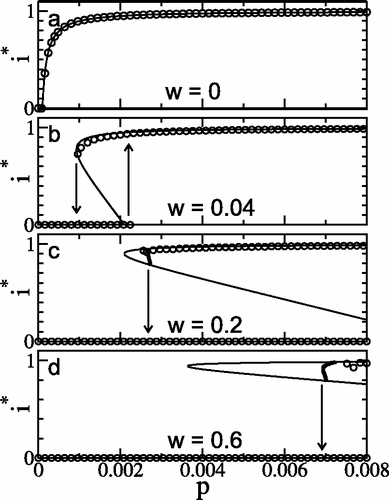
\includegraphics[width = 0.5\linewidth]{Pics/bifurcation_diagram.png}
    \caption{I 的密度作为传染概率$p^*$的函数,对于不同的重连概率$w$.}
    \label{fig:bifurcation_diagram}
\end{figure}

数值模拟表明,滞后回线和一阶跃迁的存在是自适应模型的通用特征,可以在所有有限的重连速率下观察到。虽然增加重连速率几乎不会减少局部流行病的规模,但滞后的阈值的性质会在更高的重连速率下发生变化。首先,亚临界Hopf分支产生了不稳定的极限循环,从而取代了鞍点分支。在更高的重连速率下,Hopf分支变得超临界。 由于现在出现的极限周期是稳定的,因此Hopf分叉标志着第三阈值,在该阈值处会发生连续向振荡动力学的过渡。但是,这些振荡只能在遇到持久性阈值之前在相对较小的参数区域(请参见图~\ref{fig:2-para-phase})中观察到,该阈值现在对应于循环的折叠分叉。

\begin{figure}
    \centering
    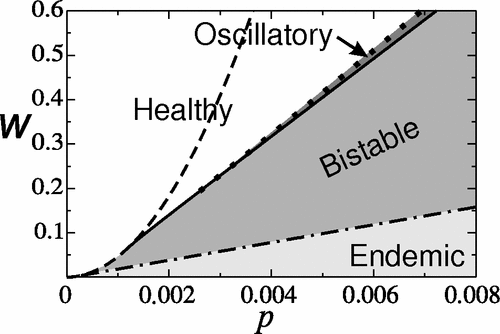
\includegraphics[width = 0.5\linewidth]{Pics/2-para-bifurcation.png}
    \caption{两个参数的相图。}
    \label{fig:2-para-phase}
\end{figure}

\section{本章Ideas}

\subsection{戴口罩的演化博弈}

\section*{演化机制}
\chapter{人类移动性}

移动性其实分为很多种,人类移动性、商品的移动性、信息的移动性都被研究了很多。Physics Reports 有一篇综述,\href{https://www.sciencedirect.com/science/article/pii/S037015731830022X}{Human mobility: Models and applications}

\section{经典模型}

王铮老师有一本书大家可以看一下,叫《理论经济地理学》里面有大量的地理学模型。虽然不算新,也没有什么实证分析,不过想法很值得借鉴。

\subsection{重力模型}

重力模型可能是地理学中最有名的模型了。形式如下:\begin{equation}
T_{i j}=\frac{m_{i}^{\alpha} n_{j}^{\beta}}{f\left(r_{i j}\right)}
\end{equation}

重力模型对火车运货量\href{https://www.jstor.org/stable/2087063?origin=crossref}{Zipf, G. K. The P 1P 2/D hypothesis: On the intercity movement of persons. Am. Sociol. Rev. 11, 677–686 (1946).}、地铁乘客\href{https://journals.aps.org/pre/abstract/10.1103/PhysRevE.86.026102}{Goh, S., Lee, K., Park, J. S. and Choi, M. Y. Modification of the gravity model and application to the metropolitan Seoul subway system. Phys. Rev. E 86, 026102 (2012).}、韩国高速公路\href{https://iopscience.iop.org/article/10.1209/0295-5075/81/48005}{Jung, W. S., Wang, F. and Stanley, H. E. Gravity model in the Korean highway. EPL 81, 48005 (2008).}、航空网络\href{https://doi.org/10.1016/j.jairtraman.2007.02.001}{Grosche, T., Rothlauf, F. and Heinzl, A. Gravity models for airline passenger volume estimation. J. Air Transp. Manag. 13, 175–183 (2007).}、通勤\href{https://science.sciencemag.org/content/312/5772/447}{Viboud, C. et al. Synchrony, waves, and spatial hierarchies in the spread of influenza. Science 312, 447–451 (2006).}和人口迁移\href{https://www.tandfonline.com/doi/abs/10.2747/0272-3638.16.4.327}{Tobler, W. Migration: Ravenstein, thornthwaite, and beyond. Urban Geogr. 16, 327–343 (1995).}等问题的拟合很不错。

通过目的地选择来推导重力模型是一个学术套路,我觉得还能玩二十年。目前目的地选择的理论有这样一些根源:确定性效用理论\href{https://doi.org/10.1111/j.1467-9787.1969.tb01340.x}{Niedercorn, J. H. and Bechdolt, B. V. Jr. An economic derivation of the "gravity law” of spatial interaction. J. Regional Sci. 9, 273–282 (1969).}、随机效用理论\href{https://www.jstor.org/stable/134305?origin=crossref}{Domencich, T. A. and  Mcfadden, D. Urban travel demand: A behavioral analysis. (North-Holland, Amsterdam, 1975).}、博弈论\href{https://www.nature.com/articles/s41598-019-46026-w}{Yan, X. Y. and Zhou, T. Destination choice game: A spatial interaction theory on human mobility. Sci. Rep. 9, 1–9 (2019).}等。文章最近也还有,不过都是集中在SR之类的期刊上。

\begin{quote}
    一个规律如果基本是客观存在且不很精确的话,不同的发现方法总是能发出文章的。毕竟人类对于规律的探索就像对孤独的回避。
\end{quote}
  
\subsection{辐射模型/介入机会(IO)模型}

辐射模型记载在Simini和Marta等人一篇名声不大好的Nature论文里,\href{https://www.nature.com/articles/nature10856}{A universal model for mobility and migration patterns. Nature 484, 96–100 (2012).}

文章中的配图甚是有意思,图一小人的表情是有出处的。法国大作家雨果写毕名著《巴黎圣母院》,与出版商有了这番史上最短通信:
\begin{center}
    “?—雨果”\\
    “!—出版商”
\end{center}

辐射模型刻画了:

辐射模型的表述如下:\begin{equation}
\left\langle T_{i j}\right\rangle=T_{i} \frac{m_{i} n_{j}}{\left(m_{i}+s_{i j}\right)\left(m_{i}+n_{j}+s_{i j}\right)}
\end{equation}其中,$T_{ij}$表示$i$到$j$的流量,$m_i$,$n_j$代表两个位置的人口,$r_{ij}$为两地距离,$s_{ij}$代表以$i$为中心,$r_{ij}$为半径的圆内的人口总数。

严小勇同志又搞了一篇Scientific Reports,\href{https://doi.org/10.1038/s41598-020-61613-y}{Liu, E., Yan, X. A universal opportunity model for human mobility. Sci Rep 10, 4657 (2020). } 介入机会(intervening opportunity)\footnote{\href{https://www.baidu.com/link?url=x-lW8LLAwVj0UCSvfYwmmsvSsLs4MiNoFonbejPvLVbktEM5xeFK2-0nwgOvZprl&wd=&eqid=b1f1d8ba0007275e000000035e8c3a1e}{Stouffer, S. A. Intervening opportunities: A theory relating mobility and distance. Am. Sociol. Rev. 5, 845–867 (1940).}}模型说的是:个体选择目的地与两个因素相关,终点的机会与起点终点之间介入的机会(?)。此类模型可以给出特定时空尺度上的准确预测,但是不同尺度上都合适的IO模型在上面这篇文章是第一次给出的。本文考虑的是人类行为的两个倾向:探索倾向和谨慎倾向。模型的形式是\begin{equation}
    {Q}_{ij}={\int }_{0}^{\infty }{\Pr }_{{m}_{i}+\alpha \cdot {s}_{ij}}(z){\Pr }_{\beta \cdot {s}_{ij}}( < z){\Pr }_{{m}_{j}}( > z)dz,
\end{equation}

\section{有意思的工作}

这个工作可以作为Allee工作的基础。

\begin{itemize}
    \item 数据源:2006年48个加拿大城市通勤普查数据,总共7 225 810人。每个城市的数据按照 census tract 组织,记录了每对职住地的人口数为$T_{ij}$. 每个 CT 约有2500-8000人居住,一般是一个城市的数个街区的大小。
\end{itemize}

CT 边界与有多少人选该CT作为工作地没有关系。记$n_{ij} = \sum_j T_{ij}$, $m_{ij} = \sum_i T_{ij}$. 将$m_j$看作随机变量,统计特征$\bar{m}$, $\sigma_m$。$W$是总工人数,$N$是城市总人口。Lloyd的平均聚集统计量:$m^* = \bar{m} + \sigma^2_m/\bar{m} - 1$ 从工作地的角度度量了工人的密度,是与随机选一个工人在同一个地方工作的工人的期望数。

\textbf{为了刻画城市间的人类移动性差异},作者动用了辐射模型。模型中,$\langle T_{ij} \rangle = p_{ij} n_{i}$其中$p_{ij}$是人取自$ij$流的概率,$n_{i}$是家处人口。利用~\cite{PhysRevE.66.016128}重的配置模型来采样。

Our model makes two assumptions: first, we assume that the spatial trajectories of humans in cities can be predicted by their home and workplace locations, which is supported by recent analyses of high-resolution data on the relocation patterns of mobile phone users [13]; second, we assume that excursions from an individual's bed or work station are governed by a stochastic process that is identically distributed across cities. 

为了实现模型,
\begin{enumerate}
    \item 先利用通勤数据来估计两地的交互频率。
    \item 将频率翻译成逐对的传播概率 $\lambda: $ the strain-specific ratio between within-hostpathogen load and transmission hazard 
\end{enumerate}

\vspace{1cm}

通勤模式分析:通勤矩阵$T_ij$的结构在城市内部和城市之间都发生了显着变化。这些可视化中的显着特征是某些城市出现了\textbf{星形}。星形形状出现在源自许多不同CT的通勤流被导向单个集中工作位置的地方。拥挤统计量$m^*$可以用来衡量城市中星型通勤模式的发生率,因为它的价值随着各个工作地点的聚集程度而增加。\begin{figure}
    \centering
    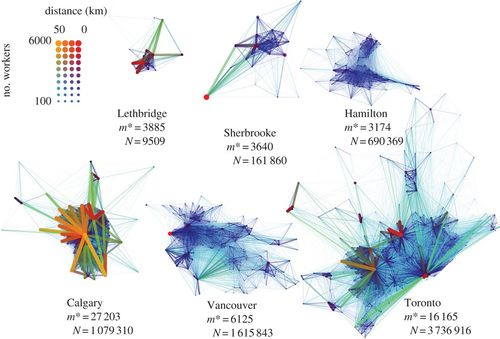
\includegraphics[width = 0.8\linewidth]{Pics/rspb20130763f01.jpg}
    \caption{城市工人的流动方式。边缘的厚度和颜色显示了CT之间上下班的人数。圆圈实际上是短边,代表生活在同一CT中的个人。较大的城市通勤模式往往井井有条,这是通过将工作站与随机选择的工人位于同一CT上的工人的平均人数来衡量的($m^*$)。但是,城市也显示出明显的组织差异,与人口规模无关。}
\end{figure}
随着总人口$N$增加,平均通勤人数$\bar{m}$很快就会饱和。相反的,$m^*$则会显示出与$N$的强烈正相关。说明大城市里的工人更倾向于前往几个巨型的工作地进行工作,但是平均每个CT中的工作地数量跟小城市差不多。所以,星形程度与在CT中工作的平均人数只是弱相关,但是与总人口关系很大。所以大城市在城市中心集中组织的程度更高。

城市还表现出明显的与大小无关的$m^*$变化,这在$m^*$随函数N回归所预测的值之比中很明显(参见电子补充材料,表S2)。在我们分析的48个城市中,$m^*/\bar{m}$(以下称为“流动性模式中的过度异质性”)介于0.43至3.07之间,相差7.14倍。对于随机选择的两个城市,的较大值和较小值之间的平均比率$m^*/\bar{m}$是1.55。在移动性模式这个尺寸无关的差相当于所预测的大小依赖性差异(基于图~\ref{rspb20130763f02} 一个),这将导致从人口尺寸的2.64倍的变化。因此,与人口规模无关的差异是城市之间工人流动模式差异的重要组成部分。
\begin{figure}
    \centering
    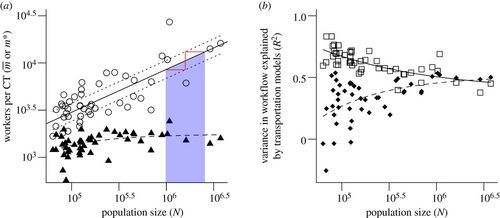
\includegraphics[width = 0.8\linewidth]{Pics/rspb20130763f02.jpg}
    \caption{Variance explained in each city by the configuration (squares) and radiation (diamonds) models of commuting flows.}
    \label{rspb20130763f02}
\end{figure}
配置模型解释了小城市通勤流量的大部分变化,但是随着N的增加,其性能会系统地下降,这表明大城市的交通方式组织化程度越来越高(图2b)。引力模型的拟合度比配置模型的拟合度差,但与大城市相比,它表现出与较小的城市更好拟合的相同趋势(请参阅电子补充材料)。辐射模型还显示出性能的系统变化:随着配置模型的适合度下降,辐射模型的性能增加,在小城市中表现相对较差,而在大城市中则更好(图2b)。

$m^*$更大代表更有条理。
\chapter{分工的形成}

分工是城市理论中的重要一环。近期的研究工作有:

\begin{itemize}
    \item  The Spatial Division of Talent in City Regions: Location Dynamics of Business Services in Copenhagen
\end{itemize}

\section{Fitness}

\href{https://www.nature.com/articles/s41586-018-0422-6}{Fitness benefits and emergent division of labour at the onset of group living}

群体生活的初始fitness的优势通常被认为是社会性演化的桎梏(要有社会性演化,先要有一点点初始的fitness)。进化理论预测这种优势需要在很小的社群中就出现。通常认为,这种优势与群体效率的标度律相关。在社会性昆虫和其他语境下,群体生活的优势被放在了相对于DOL的核心位置(DOL:个体之间的差异性,个体内部的一致性)。但是,社会性群体的“入侵”很可能很微弱,而且对于互补功能来说,相同个体数量可能是过剩的。自组织理论指出,DOL可以在很小、很简单的群体中生成。但是,关于群体规模效应作用于的DOL经验数据依然是模糊的。

本文使用长时间序列的自动化行为追踪,结合数学建模的方式,证明社会种群规模的变化可以在极度相似的,小到只有6个workers的群体中产生DOL。这些早期行为与稳态(homeostasis,保持colony和个体fitness的稳定条件)的大幅提升有关系。我们的模型指出,稳态的提升主要又与群体规模扩大相关,次要与更高度的DOL相关。我们的结果指出:DOL、稳态性提高、更高的fitness三者可以在小型同质的自然的社会族群中出现。因此,与提升社会群体规模相关的标度律才可以提升初始阶段群体生活的社会聚合力(cohesion)。
\chapter{物理模型}

\section{通过几何重正化对真实网络进行多尺度展开}

\begin{itemize}
\item
  多尺度 与 小世界 的矛盾

  \begin{itemize}
  \item
    欧式长度和对称性的缺陷
  \end{itemize}
\item
  复杂网络的几何重正化群

  \begin{itemize}
  \item
    将真实网络插入到一个度量空间,会体现出geometric scaling特征
  \end{itemize}
\end{itemize}

复杂网络中,多尺度也是共存的,但是它们被一些其他的事限制住了,并不能直接讨论\emph{自相似性}和\emph{标度无关性}。原因是我们没有一种有效的手段来对网络的length
scale进行变换。

\begin{itemize}
\item
  以前的手段:

  \begin{itemize}
  \item
    拓扑/粗粒化/random walks
  \item
    /box-covering/:证明了真实网络有着有限的分形维数,有自相似性
  \item
    拓扑scaling性质只体现在度分布、平均度、最大度上面
  \item
    尽管有很好的度量,最短路径的集合作为研究length-based scaling
    factor还是很不好的数据集。(原因是small-world的存在)
  \end{itemize}
\item
  In this work, we introduce a geometric renormalization group for
  complex networks (RGN). The method is based on a geometric embedding
  of the networks to construct renormalized versions of their structure
  by coase-graining neighbouring nodes into supernodes and defining a
  new map which progressively selects longer range connections by
  identifying relevant interactions at each scale. The RGN technique is
  inspired by the block spin renormal- ization group devised by L. P.
  Kadanoff {[}18{]}.
\end{itemize}

\subsection{真实网络中几何标度存在的证据}

研究对象:复杂网络到hidden度量空间的映射:\(\mathcal M(T,G)\)

  \begin{itemize}
  \item
    定义一个几何重正化算子$\mathbb {F_r}$,得到一个新的拓扑$T'$和一个新的几何图$G'$,由此定义一个新的重正化映射$\mathcal{M}'$: $\mathcal{M}(T,G)\stackrel{\mathbb{F_r}}{\longrightarrow}\mathcal{M}'(T',G')$
  \item
    The transformation zooms out by changing the \textbf{minimum length
    scale} from that of the original network to a larger value.
  \item
    这个过程可以迭代\(O(\ln N)\)次。
  \end{itemize}
例子:

  \begin{itemize}
  \item
    最简单的度量空间:一维圆周:\(\{\theta_i:i=1,2,3,\cdots,N\}\)

    \begin{itemize}
    \item
      重正化步骤:

      \begin{enumerate}
      \def\labelenumi{\arabic{enumi}.}
      \item
        定义block:圆周上挨着的\(r\)个点。
      \item
        粗粒化为超级结点(不管是否连接)每个超级结点都控制一个角区域。所以它们的序关系得以保留。

        \begin{itemize}
        \item
          原连接:

          \begin{itemize}
          \item
            超级结点内
          \item
            超级结点间:建立边
          \end{itemize}
        \end{itemize}
      \end{enumerate}
    \end{itemize}
  \item
    用到的例子:

    \begin{itemize}
    \item
      Internet
    \item
      Airports
    \item
      新陈代谢
    \item
      scripts\ldots\ldots{}
    \end{itemize}
  \end{itemize}
\(\mathbb S_1\)模型:将结点放在一个圆周上,以一定概率分布连接每两个点。两个点越远链接概率越低(similarity),度乘积越大连接概率越高(popularity)。

应用:The RGN enables us to unfold scale-free complex net- works in a
self-similar multi-layer shell which unveils the coexisting scales and
their interplay. Beyond

\begin{itemize}
\item
  Mini-me network replicas.

  \begin{itemize}
  \item
    networked communication systems
  \item
    可以保持微观结构的同时,不破坏介观结构
  \item
    Mini-me replicas can also be used to perform finite size scaling of
    critical phenomena taking place on real networks
  \item
    Typically, the renormalized average degree of real net- works
    increases in the flow, since they belong to the small-world phase
    (see inset in Fig. 3B), meaning that the network layer at the
    selected scale is more densely connected.
  \end{itemize}
\end{itemize}
\chapter{内卷化}

内卷化是我最近看到的一个高频词。偶然间想到这个概念与我们平时讲城市体系的层次结构似乎有着很好的对应关系,就决定在笔记里开一章做一些思考。

\bibliographystyle{unsrt}
\bibliography{ref.bib}


\end{document}


\section{\LaTeX{}的爱与恨}

今天是2020年4月17日。我终于扔掉了dndbook的模版,重新用book模版做了一个模版,并且选用了信纸作为底图。警告数从94变成了3. 请大家勤奋改模版,像我学习。